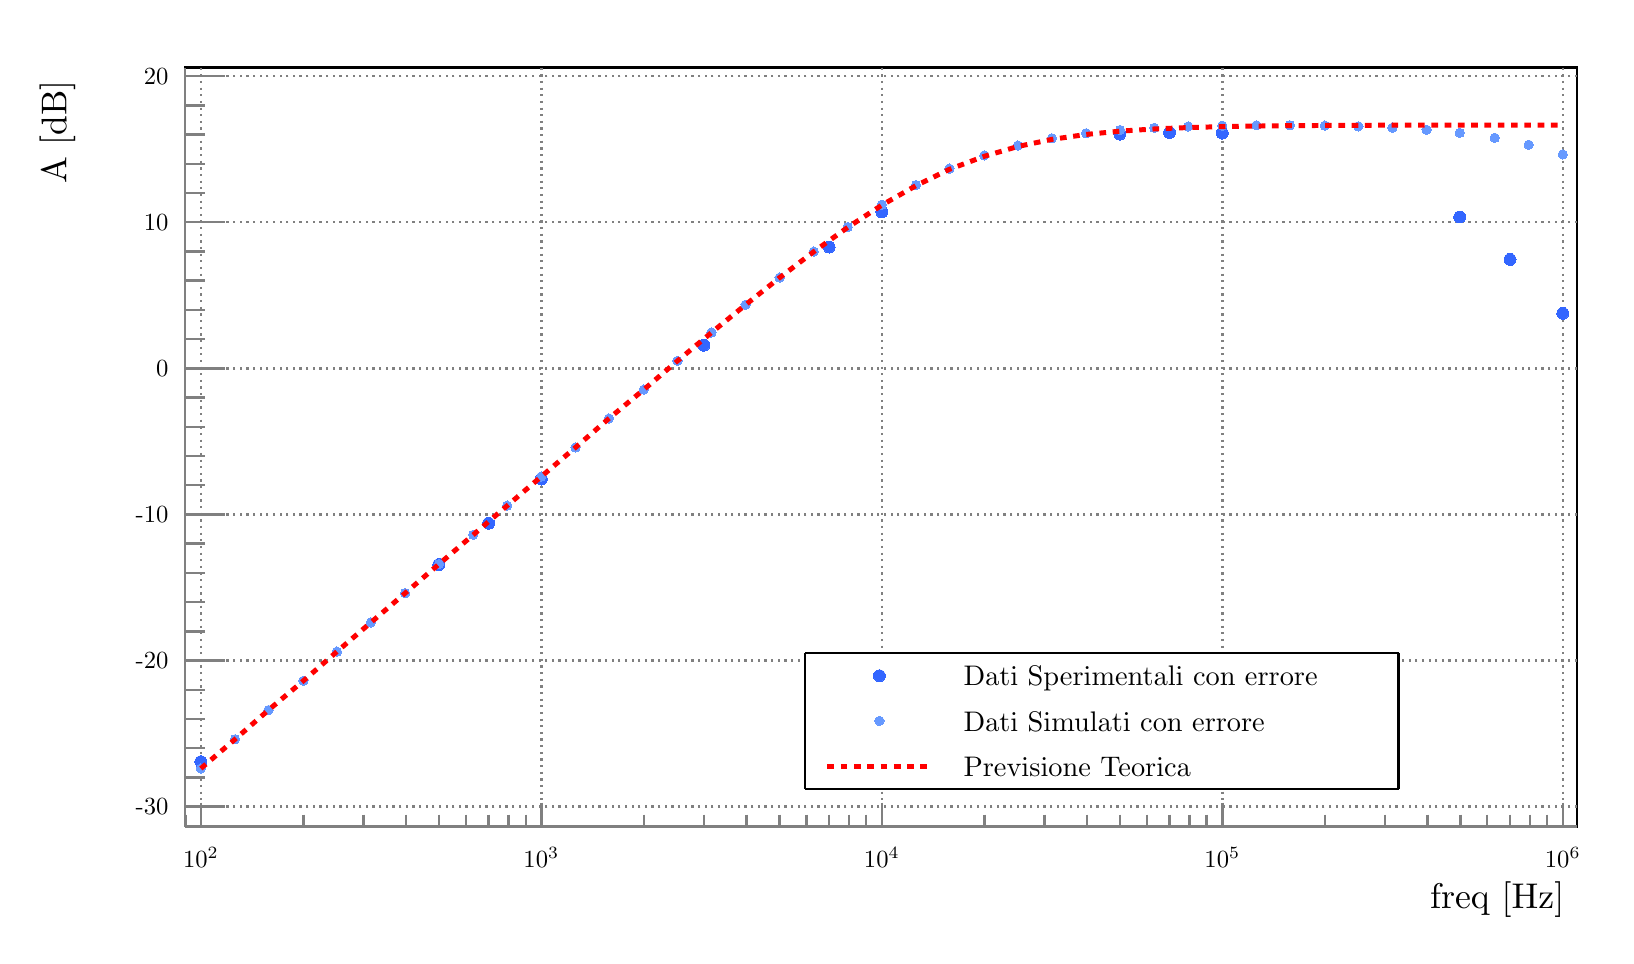
\begin{tikzpicture}
\pgfdeclareplotmark{cross} {
\pgfpathmoveto{\pgfpoint{-0.3\pgfplotmarksize}{\pgfplotmarksize}}
\pgfpathlineto{\pgfpoint{+0.3\pgfplotmarksize}{\pgfplotmarksize}}
\pgfpathlineto{\pgfpoint{+0.3\pgfplotmarksize}{0.3\pgfplotmarksize}}
\pgfpathlineto{\pgfpoint{+1\pgfplotmarksize}{0.3\pgfplotmarksize}}
\pgfpathlineto{\pgfpoint{+1\pgfplotmarksize}{-0.3\pgfplotmarksize}}
\pgfpathlineto{\pgfpoint{+0.3\pgfplotmarksize}{-0.3\pgfplotmarksize}}
\pgfpathlineto{\pgfpoint{+0.3\pgfplotmarksize}{-1.\pgfplotmarksize}}
\pgfpathlineto{\pgfpoint{-0.3\pgfplotmarksize}{-1.\pgfplotmarksize}}
\pgfpathlineto{\pgfpoint{-0.3\pgfplotmarksize}{-0.3\pgfplotmarksize}}
\pgfpathlineto{\pgfpoint{-1.\pgfplotmarksize}{-0.3\pgfplotmarksize}}
\pgfpathlineto{\pgfpoint{-1.\pgfplotmarksize}{0.3\pgfplotmarksize}}
\pgfpathlineto{\pgfpoint{-0.3\pgfplotmarksize}{0.3\pgfplotmarksize}}
\pgfpathclose
\pgfusepathqstroke
}
\pgfdeclareplotmark{cross*} {
\pgfpathmoveto{\pgfpoint{-0.3\pgfplotmarksize}{\pgfplotmarksize}}
\pgfpathlineto{\pgfpoint{+0.3\pgfplotmarksize}{\pgfplotmarksize}}
\pgfpathlineto{\pgfpoint{+0.3\pgfplotmarksize}{0.3\pgfplotmarksize}}
\pgfpathlineto{\pgfpoint{+1\pgfplotmarksize}{0.3\pgfplotmarksize}}
\pgfpathlineto{\pgfpoint{+1\pgfplotmarksize}{-0.3\pgfplotmarksize}}
\pgfpathlineto{\pgfpoint{+0.3\pgfplotmarksize}{-0.3\pgfplotmarksize}}
\pgfpathlineto{\pgfpoint{+0.3\pgfplotmarksize}{-1.\pgfplotmarksize}}
\pgfpathlineto{\pgfpoint{-0.3\pgfplotmarksize}{-1.\pgfplotmarksize}}
\pgfpathlineto{\pgfpoint{-0.3\pgfplotmarksize}{-0.3\pgfplotmarksize}}
\pgfpathlineto{\pgfpoint{-1.\pgfplotmarksize}{-0.3\pgfplotmarksize}}
\pgfpathlineto{\pgfpoint{-1.\pgfplotmarksize}{0.3\pgfplotmarksize}}
\pgfpathlineto{\pgfpoint{-0.3\pgfplotmarksize}{0.3\pgfplotmarksize}}
\pgfpathclose
\pgfusepathqfillstroke
}
\pgfdeclareplotmark{newstar} {
\pgfpathmoveto{\pgfqpoint{0pt}{\pgfplotmarksize}}
\pgfpathlineto{\pgfqpointpolar{44}{0.5\pgfplotmarksize}}
\pgfpathlineto{\pgfqpointpolar{18}{\pgfplotmarksize}}
\pgfpathlineto{\pgfqpointpolar{-20}{0.5\pgfplotmarksize}}
\pgfpathlineto{\pgfqpointpolar{-54}{\pgfplotmarksize}}
\pgfpathlineto{\pgfqpointpolar{-90}{0.5\pgfplotmarksize}}
\pgfpathlineto{\pgfqpointpolar{234}{\pgfplotmarksize}}
\pgfpathlineto{\pgfqpointpolar{198}{0.5\pgfplotmarksize}}
\pgfpathlineto{\pgfqpointpolar{162}{\pgfplotmarksize}}
\pgfpathlineto{\pgfqpointpolar{134}{0.5\pgfplotmarksize}}
\pgfpathclose
\pgfusepathqstroke
}
\pgfdeclareplotmark{newstar*} {
\pgfpathmoveto{\pgfqpoint{0pt}{\pgfplotmarksize}}
\pgfpathlineto{\pgfqpointpolar{44}{0.5\pgfplotmarksize}}
\pgfpathlineto{\pgfqpointpolar{18}{\pgfplotmarksize}}
\pgfpathlineto{\pgfqpointpolar{-20}{0.5\pgfplotmarksize}}
\pgfpathlineto{\pgfqpointpolar{-54}{\pgfplotmarksize}}
\pgfpathlineto{\pgfqpointpolar{-90}{0.5\pgfplotmarksize}}
\pgfpathlineto{\pgfqpointpolar{234}{\pgfplotmarksize}}
\pgfpathlineto{\pgfqpointpolar{198}{0.5\pgfplotmarksize}}
\pgfpathlineto{\pgfqpointpolar{162}{\pgfplotmarksize}}
\pgfpathlineto{\pgfqpointpolar{134}{0.5\pgfplotmarksize}}
\pgfpathclose
\pgfusepathqfillstroke
}
\definecolor{c}{rgb}{1,1,1};
\draw [color=c, fill=c] (0,0) rectangle (20,11.523);
\draw [color=c, fill=c] (1.96393,1.38277) rectangle (19.6393,11.022);
\definecolor{c}{rgb}{0,0,0};
\draw [c,line width=0.9] (1.96393,1.38277) -- (1.96393,11.022) -- (19.6393,11.022) -- (19.6393,1.38277) -- (1.96393,1.38277);
\definecolor{c}{rgb}{1,1,1};
\draw [color=c, fill=c] (1.96393,1.38277) rectangle (19.6393,11.022);
\definecolor{c}{rgb}{0,0,0};
\draw [c,line width=0.9] (1.96393,1.38277) -- (1.96393,11.022) -- (19.6393,11.022) -- (19.6393,1.38277) -- (1.96393,1.38277);
\definecolor{c}{rgb}{0.5,0.5,0.5};
\draw [c,line width=0.9] (1.96393,1.38277) -- (19.6393,1.38277);
\draw [c,dash pattern=on 0.80pt off 1.60pt ,line width=0.9] (2.16401,11.022) -- (2.16401,1.38277);
\draw [c,dash pattern=on 0.80pt off 1.60pt ,line width=0.9] (6.48808,11.022) -- (6.48808,1.38277);
\draw [c,dash pattern=on 0.80pt off 1.60pt ,line width=0.9] (10.8122,11.022) -- (10.8122,1.38277);
\draw [c,dash pattern=on 0.80pt off 1.60pt ,line width=0.9] (15.1362,11.022) -- (15.1362,1.38277);
\draw [c,dash pattern=on 0.80pt off 1.60pt ,line width=0.9] (19.4603,11.022) -- (19.4603,1.38277);
\draw [c,line width=0.9] (1.96393,1.38277) -- (1.96393,11.022);
\draw [c,dash pattern=on 0.80pt off 1.60pt ,line width=0.9] (19.6393,1.63644) -- (1.96393,1.63644);
\draw [c,dash pattern=on 0.80pt off 1.60pt ,line width=0.9] (19.6393,3.49214) -- (1.96393,3.49214);
\draw [c,dash pattern=on 0.80pt off 1.60pt ,line width=0.9] (19.6393,5.34784) -- (1.96393,5.34784);
\draw [c,dash pattern=on 0.80pt off 1.60pt ,line width=0.9] (19.6393,7.20353) -- (1.96393,7.20353);
\draw [c,dash pattern=on 0.80pt off 1.60pt ,line width=0.9] (19.6393,9.05923) -- (1.96393,9.05923);
\draw [c,dash pattern=on 0.80pt off 1.60pt ,line width=0.9] (19.6393,10.9149) -- (1.96393,10.9149);
\draw [c,dash pattern=on 0.80pt off 1.60pt ,line width=0.9] (19.6393,1.63644) -- (1.96393,1.63644);
\draw [c,dash pattern=on 0.80pt off 1.60pt ,line width=0.9] (19.6393,10.9149) -- (1.96393,10.9149);
\draw [c,line width=0.9] (1.96393,1.38277) -- (19.6393,1.38277);
\draw [c,line width=0.9] (1.96615,1.53552) -- (1.96615,1.38277);
\draw [c,line width=0.9] (2.16401,1.68828) -- (2.16401,1.38277);
\definecolor{c}{rgb}{0,0,0};
\draw [anchor=base] (2.16401,0.861348) node[scale=0.890168, color=c, rotate=0]{$10^{2}$};
\definecolor{c}{rgb}{0.5,0.5,0.5};
\draw [c,line width=0.9] (3.46568,1.53552) -- (3.46568,1.38277);
\draw [c,line width=0.9] (4.22712,1.53552) -- (4.22712,1.38277);
\draw [c,line width=0.9] (4.76736,1.53552) -- (4.76736,1.38277);
\draw [c,line width=0.9] (5.18641,1.53552) -- (5.18641,1.38277);
\draw [c,line width=0.9] (5.52879,1.53552) -- (5.52879,1.38277);
\draw [c,line width=0.9] (5.81827,1.53552) -- (5.81827,1.38277);
\draw [c,line width=0.9] (6.06904,1.53552) -- (6.06904,1.38277);
\draw [c,line width=0.9] (6.29022,1.53552) -- (6.29022,1.38277);
\draw [c,line width=0.9] (6.48808,1.68828) -- (6.48808,1.38277);
\definecolor{c}{rgb}{0,0,0};
\draw [anchor=base] (6.48808,0.861348) node[scale=0.890168, color=c, rotate=0]{$10^{3}$};
\definecolor{c}{rgb}{0.5,0.5,0.5};
\draw [c,line width=0.9] (7.78976,1.53552) -- (7.78976,1.38277);
\draw [c,line width=0.9] (8.55119,1.53552) -- (8.55119,1.38277);
\draw [c,line width=0.9] (9.09144,1.53552) -- (9.09144,1.38277);
\draw [c,line width=0.9] (9.51048,1.53552) -- (9.51048,1.38277);
\draw [c,line width=0.9] (9.85287,1.53552) -- (9.85287,1.38277);
\draw [c,line width=0.9] (10.1424,1.53552) -- (10.1424,1.38277);
\draw [c,line width=0.9] (10.3931,1.53552) -- (10.3931,1.38277);
\draw [c,line width=0.9] (10.6143,1.53552) -- (10.6143,1.38277);
\draw [c,line width=0.9] (10.8122,1.68828) -- (10.8122,1.38277);
\definecolor{c}{rgb}{0,0,0};
\draw [anchor=base] (10.8122,0.861348) node[scale=0.890168, color=c, rotate=0]{$10^{4}$};
\definecolor{c}{rgb}{0.5,0.5,0.5};
\draw [c,line width=0.9] (12.1138,1.53552) -- (12.1138,1.38277);
\draw [c,line width=0.9] (12.8753,1.53552) -- (12.8753,1.38277);
\draw [c,line width=0.9] (13.4155,1.53552) -- (13.4155,1.38277);
\draw [c,line width=0.9] (13.8346,1.53552) -- (13.8346,1.38277);
\draw [c,line width=0.9] (14.1769,1.53552) -- (14.1769,1.38277);
\draw [c,line width=0.9] (14.4664,1.53552) -- (14.4664,1.38277);
\draw [c,line width=0.9] (14.7172,1.53552) -- (14.7172,1.38277);
\draw [c,line width=0.9] (14.9384,1.53552) -- (14.9384,1.38277);
\draw [c,line width=0.9] (15.1362,1.68828) -- (15.1362,1.38277);
\definecolor{c}{rgb}{0,0,0};
\draw [anchor=base] (15.1362,0.861348) node[scale=0.890168, color=c, rotate=0]{$10^{5}$};
\definecolor{c}{rgb}{0.5,0.5,0.5};
\draw [c,line width=0.9] (16.4379,1.53552) -- (16.4379,1.38277);
\draw [c,line width=0.9] (17.1993,1.53552) -- (17.1993,1.38277);
\draw [c,line width=0.9] (17.7396,1.53552) -- (17.7396,1.38277);
\draw [c,line width=0.9] (18.1586,1.53552) -- (18.1586,1.38277);
\draw [c,line width=0.9] (18.501,1.53552) -- (18.501,1.38277);
\draw [c,line width=0.9] (18.7905,1.53552) -- (18.7905,1.38277);
\draw [c,line width=0.9] (19.0413,1.53552) -- (19.0413,1.38277);
\draw [c,line width=0.9] (19.2625,1.53552) -- (19.2625,1.38277);
\draw [c,line width=0.9] (19.4603,1.68828) -- (19.4603,1.38277);
\definecolor{c}{rgb}{0,0,0};
\draw [anchor=base] (19.4603,0.861348) node[scale=0.890168, color=c, rotate=0]{$10^{6}$};
\draw [anchor= east] (19.6393,0.460922) node[scale=1.29074, color=c, rotate=0]{freq [Hz]};
\definecolor{c}{rgb}{0.5,0.5,0.5};
\draw [c,line width=0.9] (1.96393,1.38277) -- (1.96393,11.022);
\draw [c,line width=0.9] (2.46584,1.63644) -- (1.96393,1.63644);
\draw [c,line width=0.9] (2.21488,2.00758) -- (1.96393,2.00758);
\draw [c,line width=0.9] (2.21488,2.37872) -- (1.96393,2.37872);
\draw [c,line width=0.9] (2.21488,2.74986) -- (1.96393,2.74986);
\draw [c,line width=0.9] (2.21488,3.121) -- (1.96393,3.121);
\draw [c,line width=0.9] (2.46584,3.49214) -- (1.96393,3.49214);
\draw [c,line width=0.9] (2.21488,3.86328) -- (1.96393,3.86328);
\draw [c,line width=0.9] (2.21488,4.23442) -- (1.96393,4.23442);
\draw [c,line width=0.9] (2.21488,4.60556) -- (1.96393,4.60556);
\draw [c,line width=0.9] (2.21488,4.9767) -- (1.96393,4.9767);
\draw [c,line width=0.9] (2.46584,5.34784) -- (1.96393,5.34784);
\draw [c,line width=0.9] (2.21488,5.71897) -- (1.96393,5.71897);
\draw [c,line width=0.9] (2.21488,6.09011) -- (1.96393,6.09011);
\draw [c,line width=0.9] (2.21488,6.46125) -- (1.96393,6.46125);
\draw [c,line width=0.9] (2.21488,6.83239) -- (1.96393,6.83239);
\draw [c,line width=0.9] (2.46584,7.20353) -- (1.96393,7.20353);
\draw [c,line width=0.9] (2.21488,7.57467) -- (1.96393,7.57467);
\draw [c,line width=0.9] (2.21488,7.94581) -- (1.96393,7.94581);
\draw [c,line width=0.9] (2.21488,8.31695) -- (1.96393,8.31695);
\draw [c,line width=0.9] (2.21488,8.68809) -- (1.96393,8.68809);
\draw [c,line width=0.9] (2.46584,9.05923) -- (1.96393,9.05923);
\draw [c,line width=0.9] (2.21488,9.43036) -- (1.96393,9.43036);
\draw [c,line width=0.9] (2.21488,9.8015) -- (1.96393,9.8015);
\draw [c,line width=0.9] (2.21488,10.1726) -- (1.96393,10.1726);
\draw [c,line width=0.9] (2.21488,10.5438) -- (1.96393,10.5438);
\draw [c,line width=0.9] (2.46584,10.9149) -- (1.96393,10.9149);
\draw [c,line width=0.9] (2.46584,1.63644) -- (1.96393,1.63644);
\draw [c,line width=0.9] (2.46584,10.9149) -- (1.96393,10.9149);
\definecolor{c}{rgb}{0,0,0};
\draw [anchor= east] (1.86393,1.63644) node[scale=0.890168, color=c, rotate=0]{-30};
\draw [anchor= east] (1.86393,3.49214) node[scale=0.890168, color=c, rotate=0]{-20};
\draw [anchor= east] (1.86393,5.34784) node[scale=0.890168, color=c, rotate=0]{-10};
\draw [anchor= east] (1.86393,7.20353) node[scale=0.890168, color=c, rotate=0]{0};
\draw [anchor= east] (1.86393,9.05923) node[scale=0.890168, color=c, rotate=0]{10};
\draw [anchor= east] (1.86393,10.9149) node[scale=0.890168, color=c, rotate=0]{20};
\draw [anchor= east] (0.342685,11.022) node[scale=1.29074, color=c, rotate=90]{A [dB]};
\definecolor{c}{rgb}{0.2,0.4,1};
\foreach \P in {(2.16401,2.20801), (5.18641,4.71175), (5.81828,5.23628), (6.48809,5.79769), (8.55119,7.49686), (10.1424,8.74416), (10.8122,9.189), (13.8346,10.178), (14.4664,10.1984), (15.1362,10.1908), (18.1516,9.12562), (18.7905,8.58678),
 (19.4603,7.90194)}{\draw[mark options={color=c,fill=c},mark size=2.162162pt, line width=0.000000pt, mark=*] plot coordinates {\P};}
\definecolor{c}{rgb}{0.4,0.6,1};
\foreach \P in {(2.16401,2.12145), (2.59802,2.49257), (3.02302,2.86368), (3.46569,3.23477), (3.89223,3.60584), (4.3247,3.97686), (4.75795,4.34782), (5.19016,4.71867), (5.6234,5.08935), (6.0549,5.45977), (6.48809,5.82976), (6.9221,6.19909),
 (7.34709,6.56737), (7.78976,6.93399), (8.2163,7.29802), (8.64877,7.65802), (9.08203,8.01182), (9.51424,8.35622), (9.94747,8.68671), (10.379,8.99736), (10.8122,9.28104), (11.2462,9.5305), (11.6712,9.73997), (12.1138,9.90707), (12.5404,10.0336),
 (12.9728,10.125), (13.4061,10.1883), (13.8383,10.2307), (14.2715,10.2583), (14.7031,10.2755), (15.1362,10.2855), (15.5702,10.2901), (15.9952,10.2903), (16.4379,10.2861), (16.8645,10.2767), (17.2969,10.2602), (17.7302,10.2338), (18.1516,10.1943),
 (18.5956,10.1318), (19.0271,10.0433), (19.4603,9.92016)}{\draw[mark options={color=c,fill=c},mark size=1.681682pt, line width=0.000000pt, mark=*] plot coordinates {\P};}
\definecolor{c}{rgb}{1,0,0};
\draw [c,dash pattern=on 2.40pt off 2.40pt ,line width=1.8] (2.16401,2.12145) -- (2.59802,2.49257) -- (3.02302,2.86368) -- (3.46569,3.23477) -- (3.89223,3.60584) -- (4.3247,3.97686) -- (4.75795,4.34781) -- (5.19016,4.71866) -- (5.6234,5.08933) --
 (6.0549,5.45973) -- (6.48809,5.8297) -- (6.9221,6.19898) -- (7.34709,6.5672) -- (7.78976,6.93372) -- (8.2163,7.2976) -- (8.64877,7.65736) -- (9.08203,8.0108) -- (9.51424,8.35465) -- (9.94747,8.68434) -- (10.379,8.99387) -- (10.8122,9.2761) --
 (11.2462,9.52378) -- (11.6712,9.73129) -- (12.1138,9.89645) -- (12.5404,10.0213) -- (12.9728,10.1113) -- (13.4061,10.1738) -- (13.8383,10.2159) -- (14.2715,10.2436) -- (14.7031,10.2616) -- (15.1362,10.2731) -- (15.5702,10.2805) -- (15.9952,10.2852)
 -- (16.4379,10.2882) -- (16.8645,10.2901) -- (17.2969,10.2913) -- (17.7302,10.292) -- (18.1624,10.2925) -- (18.5956,10.2928) -- (19.0271,10.293) -- (19.4603,10.2931);
\definecolor{c}{rgb}{1,1,1};
\draw [color=c, fill=c] (9.83968,1.86373) rectangle (17.3748,3.58717);
\definecolor{c}{rgb}{0,0,0};
\draw [c,line width=0.9] (9.83968,1.86373) -- (17.3748,1.86373);
\draw [c,line width=0.9] (17.3748,1.86373) -- (17.3748,3.58717);
\draw [c,line width=0.9] (17.3748,3.58717) -- (9.83968,3.58717);
\draw [c,line width=0.9] (9.83968,3.58717) -- (9.83968,1.86373);
\draw [anchor=base west] (11.7234,3.17067) node[scale=1.02369, color=c, rotate=0]{Dati Sperimentali con errore};
\definecolor{c}{rgb}{0.2,0.4,1};
\foreach \P in {(10.7816,3.29993)}{\draw[mark options={color=c,fill=c},mark size=2.162162pt, line width=0.000000pt, mark=*] plot coordinates {\P};}
\definecolor{c}{rgb}{0,0,0};
\draw [anchor=base west] (11.7234,2.59619) node[scale=1.02369, color=c, rotate=0]{Dati Simulati con errore};
\definecolor{c}{rgb}{0.4,0.6,1};
\foreach \P in {(10.7816,2.72545)}{\draw[mark options={color=c,fill=c},mark size=1.681682pt, line width=0.000000pt, mark=*] plot coordinates {\P};}
\definecolor{c}{rgb}{0,0,0};
\draw [anchor=base west] (11.7234,2.02171) node[scale=1.02369, color=c, rotate=0]{Previsione Teorica };
\definecolor{c}{rgb}{1,0,0};
\draw [c,dash pattern=on 2.40pt off 2.40pt ,line width=1.8] (10.1222,2.15097) -- (11.4409,2.15097);
\end{tikzpicture}
